%\placelogofalse
\begin{frame}{Poisson's Equation}
\begin{columns}
\column{0.58\linewidth}
$$ - \Delta u = f \text{ in } \Omega, u = f(x, y, z) \text{ on } \nabla \Omega
$$

Multiply both sides by a \textit{test function} $v$

Integrate over the domain $\Omega$

$$
\int_{\Omega}(-Delta u) v \ dx = \int_{\Omega} f v \ dx
$$

Apply integration by parts to move derivatives off of $u$ , such that $u \in H^1$, not $C^2$.

$$
\int_{\Omega} \nabla u \cdot \nabla v dx = \int_{\Omega} f v \ dx
$$


\textit{Variation Form}
Find $u \in V$ such that

$$
a(u, v) = L(v) \ \forall v \in V,
$$
Where
\begin{align*}
  a(u, v) &= \int_{\Omega} \nabla u \cdot v \ dx \text{ Bilinear form} \\
  L(v) &= \int_{\Omega} f  \ dx \text{ Linear Form}
\end{align*}

\column{0.38\linewidth}
\begin{center}
\centering
%\shadowimage[width=2.5cm]{example_1.png}

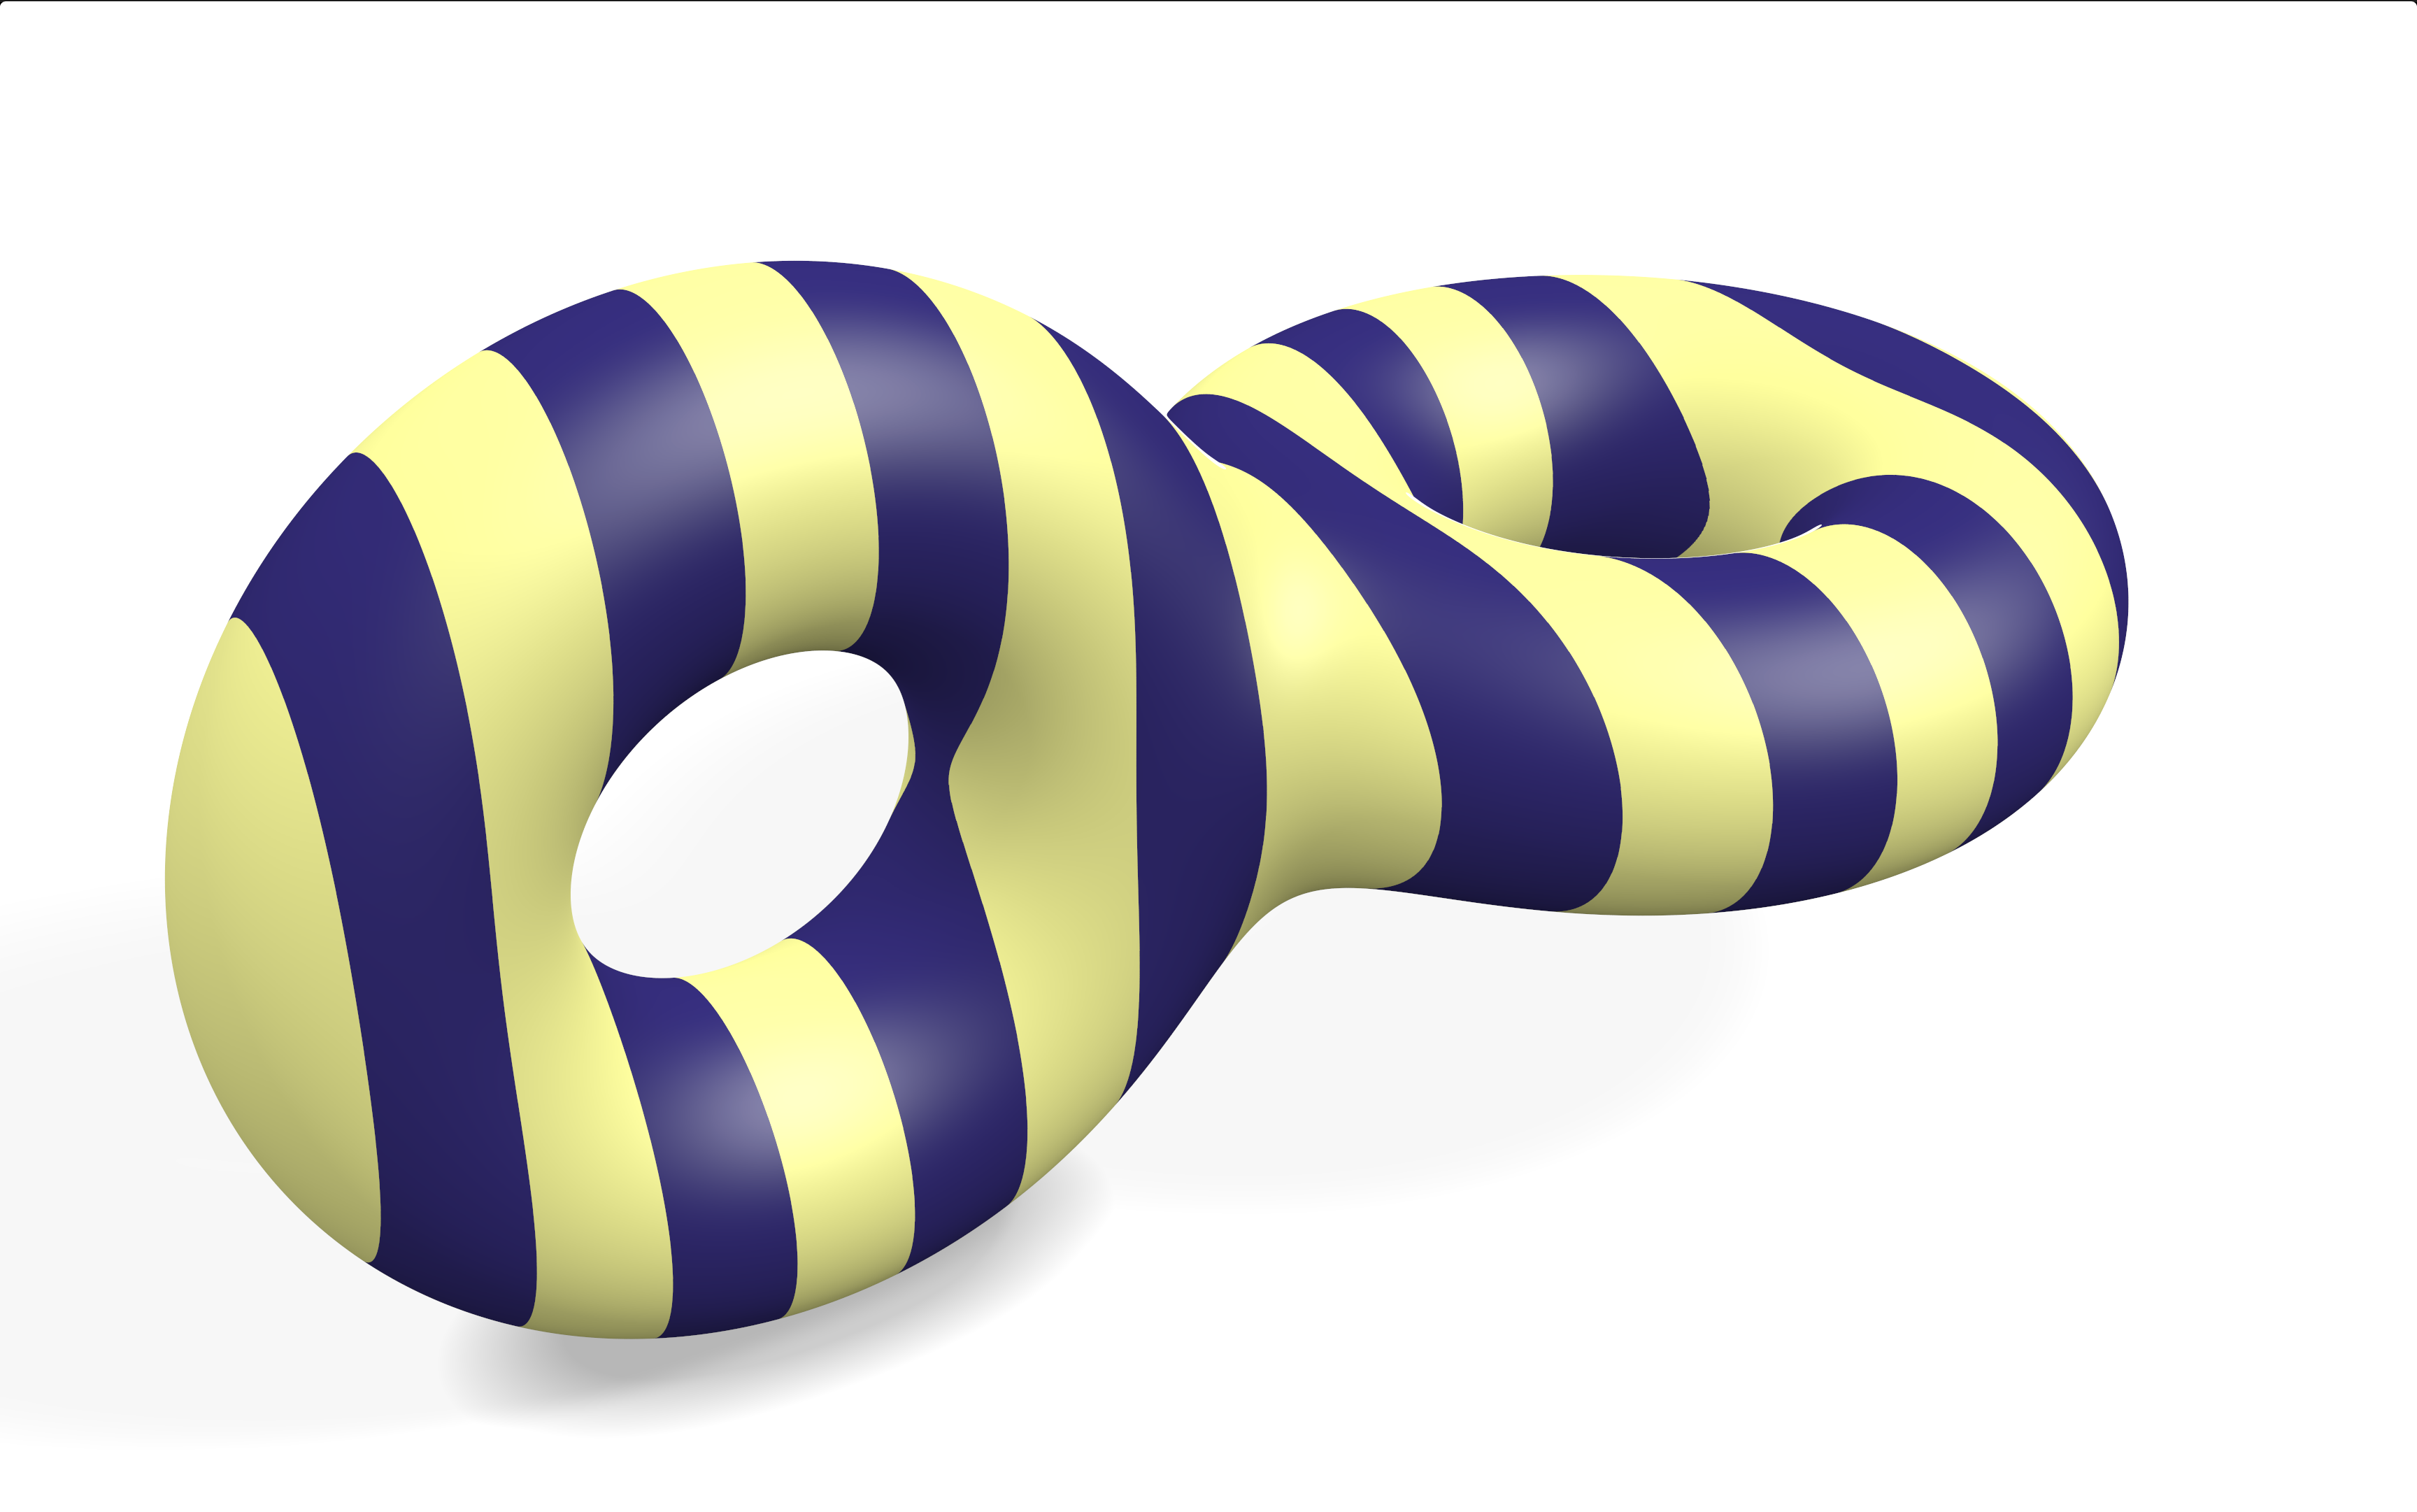
\includegraphics[width=2.5cm]{assets/poisson_1.png}

\vspace{0.2cm}

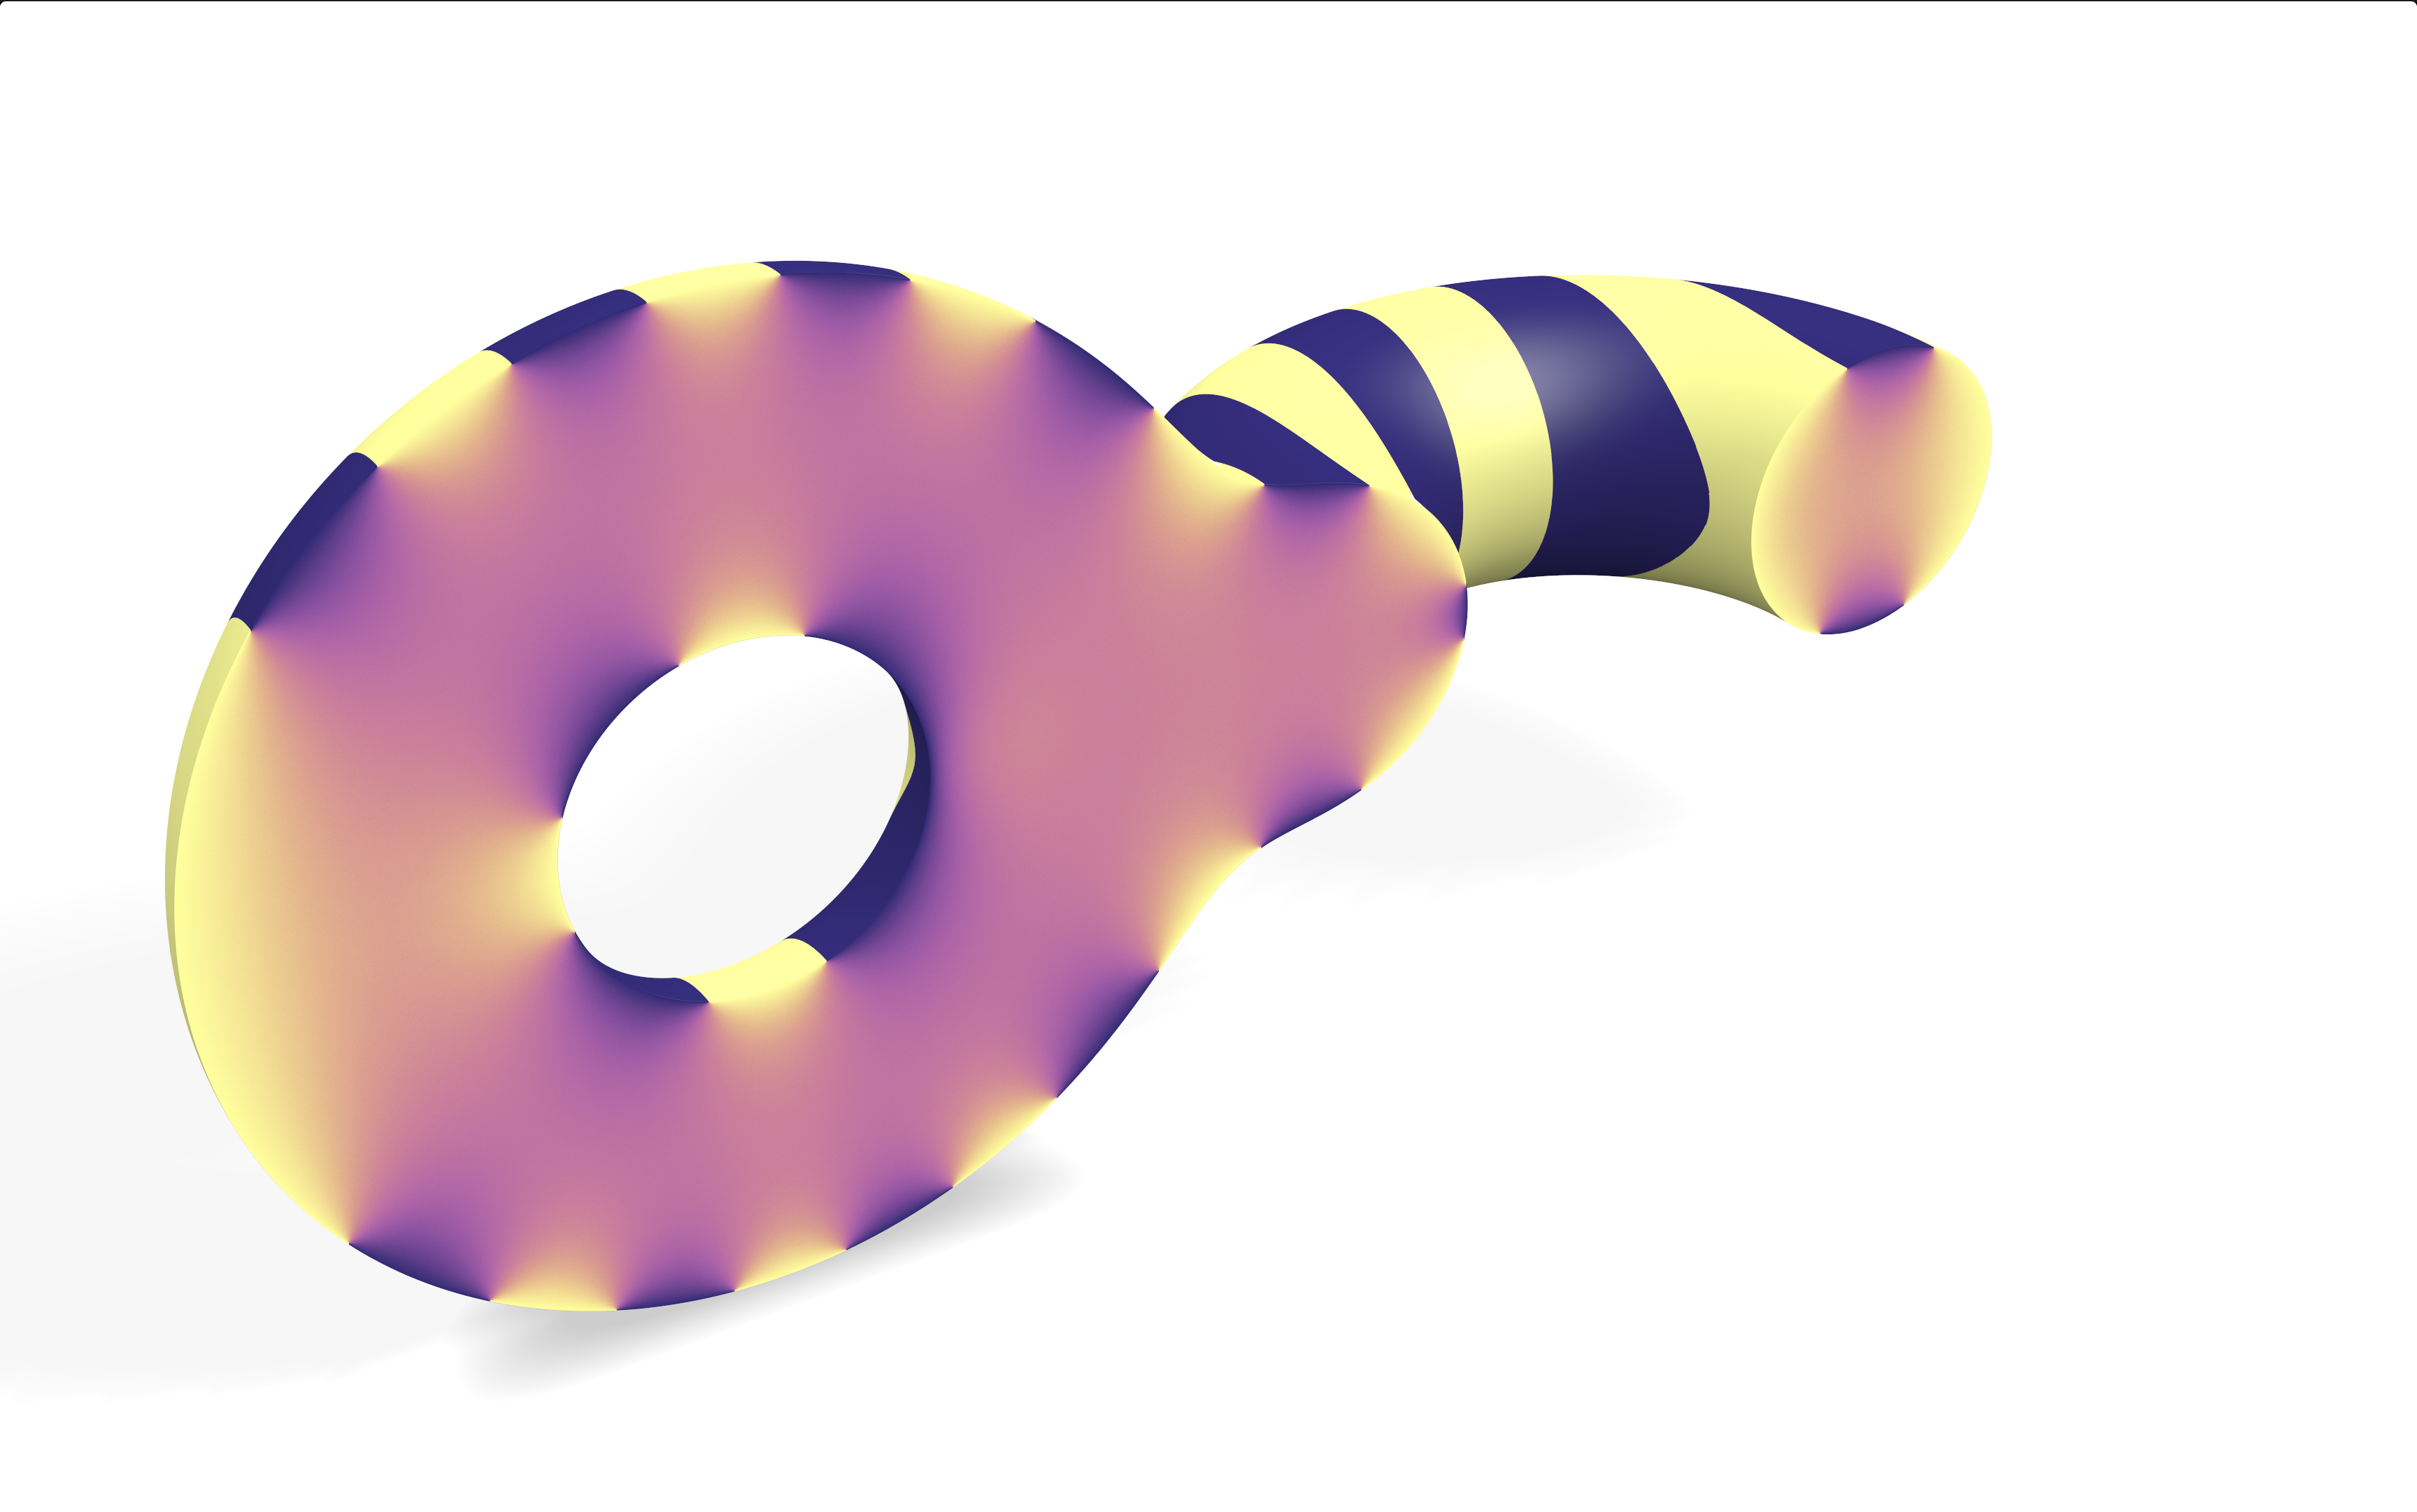
\includegraphics[width=2.5cm]{assets/poisson_2.png}


% [trim={left bottom right top},clip]
%
\includegraphics[width=8.5cm, page=3, trim={0 9cm 14cm 0cm},clip]{assets/vec_db_figs.pdf}
\end{center}
\end{columns}
\end{frame}
%\placelogotrue

\begin{frame}[fragile]{Python Example}
\begin{lstlisting}[language=Python]
from ufl import *

# Mesh and function space (provided by higher-level FEniCS code, not UFL itself)
V = FunctionSpace(mesh, "Lagrange", 1)

u = TrialFunction(V)   # unknown
v = TestFunction(V)    # test function
f = Function(V)        # source term

a = dot(grad(u), grad(v)) * dx
L = f * v * dx
\end{lstlisting}
\end{frame}

%\placelogofalse
\begin{frame}{Poisson Problem: Finite Element Discritization Pt1}
  \begin{align*}
    -\Delta u &= f \text{ in } \Omega \\
    -\Delta u v &= f v \text { in } \Omega \\
    \int_{\Omega} \nabla u \cdot \nabla v \ dx
    - \int_{\partial \Omega} \partial_n u v \ ds 
                &= \int_{\Omega} f v \ dx \\
   \int_{\Omega} \nabla u \cdot \nabla v \ dx
                &= \int_{\Omega} f v \ dx 
                - \int_{\Gamma_N} g v \ ds \ \forall v \in \hat{V}\\
  \end{align*}
\end{frame}
%\placelogotrue

\begin{frame}{Poisson Problem: Finite Element Discritization Pt2}
  \begin{align*}
    u_h(x) &= \sum^N_{j = 1} U_j \phi_j(x) \\
    \sum^N_{j = 1} U_j \int_{\Omega} \nabla \phi_j \cdot \nabla \hat{\phi}_i \ dx &= \int_{\Omega} f \hat{\phi}_i \ dx - \int_{\Gamma_N} g \hat{\phi}_i \ ds \ i = 1, 2, \cdots, N
  \end{align*}
  Compute FE solution $u_h = \sum^N_{j = 1} U_j \phi_j$ by solving
  $$AU = b$$
  where
\begin{align*}
  A_{ij} &= \int_{\Omega} \nabla \phi_j \cdot \nabla \hat{\phi}_i \ dx \\
  b_i &= \int_{\Omega} f \hat{\phi}_i \ dx - \int_{\Gamma_N} g \hat{\phi}_i \ ds 
\end{align*}
\end{frame}

\begin{frame}{Solve Step}
  \begin{outline}
    \1 Explain linear solver / sparsity pattern / solution viewing on mesh
  \end{outline}
\end{frame}

\begin{frame}{Integrating with Quadrature}
\begin{align*}
  A_{ij} &= \int_{\Omega} \nabla \phi_j \cdot \nabla \hat{\phi}_i \ dx \\
         &\approx \sum_{k = 1}{K} w_k \nabla \phi_j(x_k) \cdot \nabla \hat{\phi}_i (x_k)
\end{align*}
\begin{outline}
  \1 Explain integration with quadrature rules 
\end{outline}
\end{frame}

\begin{frame}{Implementating this}
  \begin{outline}
    \1 Show and explain integrator from intact
  \end{outline}
\end{frame}

\begin{frame}[fragile]{UFL}
  \begin{columns}
    \column{0.48\linewidth}
  \begin{outline}
    \1 Look at how we can model this in UFL
  \end{outline}

  \column{0.48\linewidth}
  \begin{lstlisting}[language=Python]
u = ufl.TrialFunction(V)
v = ufl.TestFunction(V)
x = ufl.SpatialCoordinate(msh)
f = <source expression> 
g = ufl.sin(5 * x[0])
a = inner(grad(u), grad(v)) * dx
L = inner(f, v) * dx * ds
  \end{lstlisting}
  \end{columns}
\end{frame}

\begin{frame}{Demo}
Demo FENICS code
\end{frame}

\begin{frame}{Variational Forms}
Explain variation forms from paper in general
\end{frame}

\begin{frame}{Symbollic Represenation}
  Build expression tree in python
\end{frame}

\begin{frame}{Code generation}
  Adopted by other projects
  Form Compiler in FENICS
\end{frame}

\begin{frame}{Research with UFL}
  What are people doing with it?
\end{frame}

\begin{frame}{Get to conclusion?}
  Discussion points
\end{frame}
